\section{Limiting GP for the Deep Manifold Prior}\label{sec:gp}
\begin{figure*}[t]
\centering
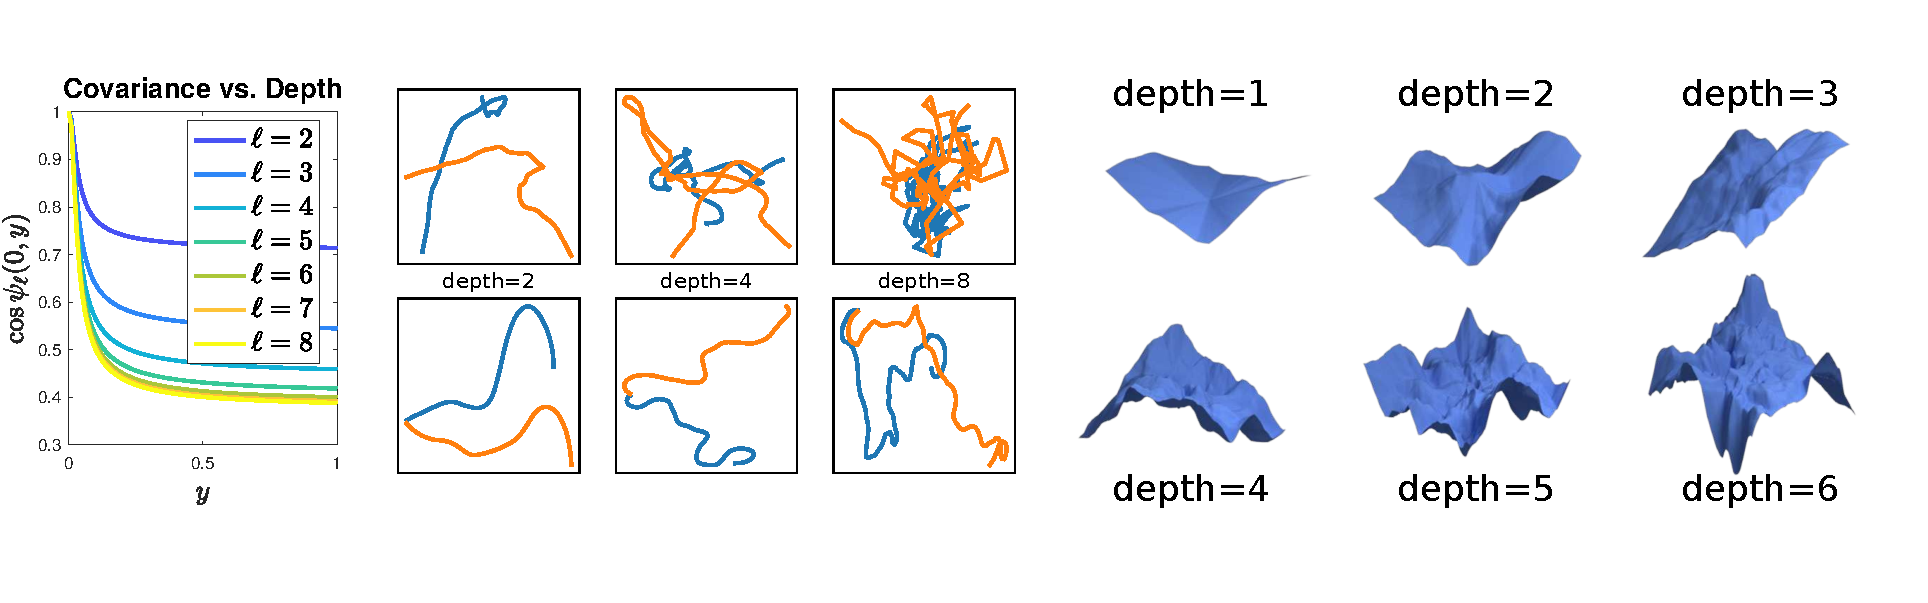
\includegraphics[width=\linewidth]{dmp/imgs/priorsamples.pdf}
\vspace{-30pt}
\caption{\label{fig:priorsamples} \small
  \textbf{Characterizing the deep manifold prior.}
  \textbf{(left)} a plot demonstrating the relationship between the network
  depth and the covariance function for the limiting GP. \textbf{(middle)}
  Random curves generated by the coordinate (top rows) and arc-length (bottom rows) parametrizations using deep networks with varying depths. \textbf{(right)} Random surfaces generated by deep networks of varying depths.} 
\end{figure*}

Consider the case when the manifold coordinates are parametrized using a deep network 
$f_\theta(x)$.
We show that random networks, \eg, whose 
parameters are drawn i.i.d. from a Gaussian distribution, produces smooth manifolds.
This is done by analyzing the limiting behavior of the function as a Gaussian
process.
In practice this is a good approximation to networks that are
relatively shallow and have hundreds of hidden units in each layer.

Concretely, the mean $\mathbb{E}_\theta[f_\theta(x)]$ and covariance
$\mathbb{E}_\theta[f_\theta(x) f_\theta(y)^T]$ of the parameterization 
characterize the structure of the generated manifold. 
For example, the covariance function of a smooth manifold decays
slowly as a function of distance in the input space compared to
a rough one.
Following prior work~\cite{Neal,williams1997computing,cho2009kernel},
we first derive the mean and covariance for a two layer network with a 
scalar output. We then generalize the analysis to vector outputs and multi-layer
networks.

Consider a two-layer fully-connected network on an input $x \in \mathbb{R}^n$. 
Let $H$ be the number of units in the hidden layer
represented using parameters $U = (u_1, u_2, \ldots u_H)$ where $u_j \in \mathbb{R}^n$
and the second layer has one output parameterized by weights $v \in
\mathbb{R}^H$. Denote the non-linearity applied to each unit as the
scalar function $h(\cdot)$. The output of the network is:  $f(x) = \sum_{k=1}^{H} v_k h(u_k^Tx).$
When the parameters $U$ and $v$ are
drawn from a Gaussian distributions $N(0, \sigma_u^2\mathbb{I})$ and
$N(0, \sigma_v^2\mathbb{I})$ respectively, we have:
\begin{equation*}
\mathbb{E}_{U,v}[f(x)] = \mathbb{E}_{U,v} \left[ \sum_{k=1}^{H} v_k
  h\left(u_k^Tx\right)\right] = 0, 
\end{equation*}
since $U$ and $v$ are independent and zero mean. 
Similarly, the covariance function $K(x,y)$ can be shown to be:
\begin{align*}
K(x,y) = \mathbb{E}_{U,v}[f(x)f(y)] = H\sigma_v^2 \mathbb{E}_{U} \left[ h\left(u_k^Tx\right)
  h\left(u_k^Ty\right) \right].
\end{align*}
This follows since each $u_k$ is drawn i.i.d, each
$v_k$ is independent and drawn identically from a Gaussian
distribution with zero mean.
The quantity $V(x, y)=E_u \left[ h(u^Tx)h(u^Ty)\right]$ can be
computed analytically for various transfer functions. 
Williams~\cite{williams1997computing} showed that when $h(t) = {\rm erf}(t) =
2/\sqrt{\pi}\int_{0}^{t}e^{-t^2}dt$, then 
\begin{align}
V_{{\rm erf}}(x, y) = \frac{2}{\pi}\sin^{-1} \frac{x^T\Sigma
  y}{\sqrt{\left(x^T\Sigma x \right)\left(y^T\Sigma y\right)}}. 
\end{align}
Here $\Sigma=\sigma^2 \mathbb{I}$ is the covariance of $u$.
For the ReLU non-linearity $h(t) = \max(0,t)$, Cho and Saul~\cite{cho2009kernel}
derived the expectation as:
\begin{align}
V_{\rm relu}(x, y) = \frac{1}{\pi}\Vert x \Vert \Vert y \Vert
\left(\sin \psi + (\pi -\psi)\cos \psi \right), 
\end{align}
where $\psi = \cos^{-1}\left(\frac{x^Ty}{\Vert x \Vert  \Vert y
  \Vert}\right)$. We refer the reader to~\cite{williams1997computing,cho2009kernel} for kernels
corresponding of other transfer functions.

An application of the Central Limit Theorem shows that by letting $\sigma_v^2$ scale as $1/H$ and $H \rightarrow \infty$,
the output of a two layer convolutional network converges to a
Gaussian distribution with zero mean and covariance 
\begin{align}
  K_1(x, y) = E_{U,v} \left[ f(x)f(y)\right] = V\left(x,y\right).
\end{align}

Hence the limiting behavior of the DNN can be approximated as a
Gaussian process with a zero mean and covariance function $K(x,y) =
V(x,y)$.

\paragraph*{Extending to multiple outputs} The above analysis can be
extended to the case when the function $f(x)$ is vector
valued. For example a 2-manifold in 3D can be represented as $f(x) = (f^1(x), f^2(x), f^3(x))$, with $x \in \mathbb{R}^2$. 
In our case, the functions share a common backbone and each $f^i(x)$ is constructed from the outputs of the last hidden layer parameterized with
weights $v^i$, \ie, $f^i(x) = \sum_{k=1}^{H} v_k^i h(u_k^Tx).$
From the earlier analysis we have that each $f^i(x)$ has zero mean in
expectation. 
And the covariance between dimension $i$ and $j$ of $f$ is:
\begin{align*}
K_{1}^{i,j}(x,y) = \mathbb{E}_{U,v_i, v_j} \left[ f^i(x)f^j(y)\right] = V\left(x,y\right) \mathbf{1}[i=j].
\end{align*}
This follows from the fact that each $v_k^i$ is independent and drawn
from a zero mean distribution. 
Thus, the covariance is a diagonal matrix with entries $V(x,y)$ 
in its the diagonal.

\paragraph*{Extending to multiple layers}
The analysis can be extended to multiple
layers by recursively applying the formula for the two-layer network.
Denote $K_\ell(x,y)$ as the covariance function of a scalar valued
fully-connected network with $\ell+1$ layers and $J(\theta) = \sin \theta
+ (\pi-\theta) \cos \theta$. Following~\cite{cho2009kernel} for the ReLU non-linearity we have the
following recursion:
\begin{align*}
K_{\ell+1}(x,y) = \frac{1}{\pi}\left(K_{\ell}(x,x) K_{\ell}(y,y)\right)^{1/2} J\left(\psi_{\ell}\right).
\end{align*}
Where $\psi_\ell(x,y) = \cos^{-1}
\frac{K_\ell(x,y)}{\sqrt{K_\ell(x,x)K_\ell(y,y)}}$ and $K_{0}(x,y) =
x^Ty$. Note that if in each layer we add a bias term sampled from a $N(0,
\sigma_b^2)$ the covariance changes to $K_\ell(x,y)
+ \sigma_b^2$ and the mean remains unchanged at zero. 

\subsection{Discussion and Analysis}
The above analysis shows that random networks induce certain priors
over the coordinates of the manifold. 
The effect of increasing the depth of the network can be seen by
visualizing how the covariance 
$\cos \psi_\ell (x, y)$ varies as a function of depth.
Figure~\ref{fig:priorsamples} plots $\cos \psi_\ell (x, y)$
at $x=0$ for a curve as a function of the depth of the network for
$\sigma_b=0.01$.
The covariance decays faster with depth, indicating
that the deeper networks produce manifolds with higher spatial frequencies (or curvatures).
This can also be seen in Figure~\ref{fig:priorsamples} which shows random curves (middle) from a
surfaces (right) for networks with varying depths. 

One potential drawback of fully-connected network parameterization is that the
generated manifold does not have a stationary (translationally invariant) covariance function. 
A covariance function $K(x,y)$ is stationary if it can be written as
$K(x,y) = k(x-y)$. 
On the other hand, a convolutional network that produces coordinates through a series of convolutional layers operating on
a random noise has a stationary covariance~\cite{cheng2019bayesian}. 
This is identical to the approach for generating natural images in the
deep image prior~\cite{dip} and we explore this alternative in Section~\ref{sec:exp_data}.

\paragraph*{Normals and curvature} While we have shown that the outputs $f(x)$ induced by
random networks is a GP in the limit, what can be said about intrinsic properties
such as normals and curvature? 
Consider the curve $\gamma(t) = (x(t), y(t))$. 
Since derivatives are linear operators, it follows that 
distribution of derivatives, $\dot{x}$ and $\dot{y}$, are also Gaussian~\cite{solak2003derivative}.
The curvature is given by $\kappa = (\ddot{x}\dot{y} - \ddot{y}\dot{x})/(\dot{x}^2 + \dot{y}^2)^\frac{3}{2}.$
Unfortunately, since each of the derivatives converge to a zero mean
Gaussian distribution, the limiting distribution of the curvature $\kappa$ does
not exist. 
The pathology arises because the parameterization has a
speed ambiguity, \ie, replacing $t$
with any monotonic function of $t$ results in the same curve. 
To avoid this one can directly parametrize the derivatives as $\dot{x} =
\cos(f(t))$ and $\dot{y} = \sin(f(t))$ where $f$ is a deep network.
This is an arc-length (unit speed) parametrization since $\dot{x}^2 + \dot{y}^2 = 1$.
Once the derivatives are generated, the curve can be reconstructed by integration, \ie, $x = \int_0^t \cos(f(t)) dt$.
In this case the limiting distribution of the coordinates, normal, and
curvature all exist and are also GPs. We derive the mean and
covariance function in the Supplementary material.
Figure~\ref{fig:priorsamples}-middle shows draws from the GP with direct (top) and arc-length (bottom) parametrizations. 
One can see that arc-length parametrizations lead to more length-uniform curves.

Unlike curves, it is much more challenging to design arc-length parametrizations of surfaces. 
The difficulty arises due to the fact the gradients need to satisfy additional constraints for the surface to be
integrable~\cite{sussmann1973orbits}. 
Hence, we directly parameterized the coordinate function and proposed the stretch regularization to minimize distortion.
Alternatives ways of parameterizing the surface to satisfy properties such as conformality~\cite{nehari2012conformal} is left for future work.

\paragraph*{Deep level-set prior} Finally, the GP analysis applies in a straightforward manner to the level-set formation $f_\theta(x) = 0$ where $f_\theta$ is a ReLU network 
mapping the 3D position $x \in \mathbb{R}^3$ to a scalar. The induced distribution over the
scalar field is a GP for random networks. Since for a differentiable function $f$ with non-zero gradient, the gradient is orthogonal to the level set, one can characterize the surface by analyzing the gradient field $\nabla f$. The limiting distribution over the gradient field is also a GP and one can estimate the mean and convariance functions by a similar analysis (see Supplementary material for details).
However, the training objective of the level-set prior is different from the explicit parameterization as the network must classify points as inside or outside the surface. This supervision can be challenging to obtain from noisy
data, especially for thin structures. We provide a comparison with this
approach in Section~\ref{sec:experiments}. 




